% Copyright (c) 2012 by Michał Nazarewicz <mina86@mina86.com>
% Distributed under the terms of the Creative Commons
% Attribution-ShareAlike 3.0 Unported (CC BY-SA 3.0) license.

\section{Wstęp}

\subsection{Po co pamięć ciągła fizycznie?}

\begin{frame}
  \frametitle{Po co pamięć ciągła fizycznie?}
  \begin{columns}[c]

    \column{.33\textwidth}
    \begin{center}
      \includegraphics[width=\textwidth]{build/mmu-iommu-images--img-nommu.eps}
    \end{center}

    \column{.33\textwidth}
    \begin{center}
      \includegraphics[width=\textwidth]{build/mmu-iommu-images--img-dma.eps}
    \end{center}

    \column{.33\textwidth}
    \begin{center}
      \includegraphics[width=\textwidth]{build/mmu-iommu-images--img-iommu.eps}
    \end{center}

  \end{columns}
\end{frame}

\subsection{Dotychczasowe rozwiązania}

\begin{frame}
  \frametitle{Dotychczasowe rozwiązania}

  \begin{block}{Rezerwacja i~przydzielanie przy starcie systemu}
    \begin{itemize}
    \item Rezerwacja pamięci przy starcie systemu.
    \item Przypisanie na stałe buforów do urządzeń.
    \item Gdy urządzenie nic nie robi, pamięć jest marnowana.
    \end{itemize}
  \end{block}

  \begin{block}{Rezerwacja i~zarządzanie pamięcią}
    \begin{itemize}
    \item Rezerwacja pamięci przy starcie systemu.
    \item Zdefiniowanie interfejsu alokatora.
    \item Mniej pamięci jest zarezerwowanej.
    \item Niemniej nadal jest marnowana.
    \end{itemize}
  \end{block}
\end{frame}

\subsection{Proponowane rozwiązanie}

\begin{frame}
  \frametitle{Proponowane rozwiązanie}

  \begin{block}{Contiguous Memory Allocator}
    \begin{itemize}
    \item Rezerwacja pamięci przy starcie systemu.
    \item Zwracanie pamięci z~powrotem do systemu,
      \begin{itemize}
      \item ale tylko strony ruchome mogą być z~niej alokowane.
      \end{itemize}
    \item Zdefiniowanie interfejsu alokatora.
    \item Migruj strony przy alokacji.
    \end{itemize}
  \end{block}
\end{frame}


\section[Linux]{Pamięć w~Linuksie}

\subsection{Strony i~bloki stron}

\begin{frame}
  \frametitle{Strony i~bloki stron}
  \begin{center}
  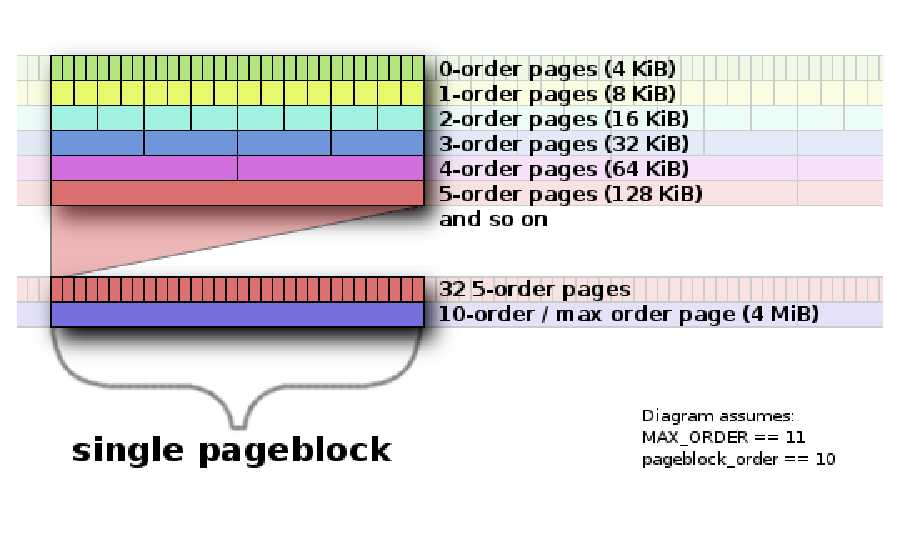
\includegraphics[width=0.9\textwidth]{build/pages.eps}
  \end{center}
\end{frame}

\subsection{Migracja stron}

\begin{frame}
  \frametitle{Typy migracji stron}

  \begin{itemize}
  \item Przy alokacji, użytkownik określa typ migracji żądanej strony:
    \textit{ruchomy} lub \textit{nieruchomy}.
  \item Każdy blok stron ma przypisany typ migracji.
  \item Przy alokacji strony są brane z~odpowiedniego bloku.
    \begin{itemize}
    \item Chyba, że takowych nie ma.
    \end{itemize}
  \item Typ bloku może się zmieniać.
  \end{itemize}
\end{frame}

\begin{frame}[fragile]
  \frametitle{Migracja}

  \begin{itemize}
  \item Strony ruchome mogą być migrowane.
  \item Migracja polega na:
    \begin{itemize}
    \item skopiowaniu zawartości strony gdzie indziej i
    \item uaktualnieniu odwołań do starej strony.
    \end{itemize}
  \item Przykładami stron ruchomych są:
    \begin{itemize}
    \item anonimowe strony procesów i
    \item bufory dyskowe.
    \end{itemize}
  \end{itemize}
\end{frame}


\section[CMA]{Implementacja CMA}

\subsection{CMA a~innye alokatory}

\begin{frame}[fragile]
  \frametitle{CMA a~innye alokatory}

  \begin{center}
    \includegraphics[width=\textwidth]{build/linux-allocators--cma.eps}
  \end{center}
\end{frame}

\subsection{Typ migracji CMA}

\begin{frame}
  \frametitle{Typ migracji CMA}

  \begin{itemize}
  \item CMA migruje wiele stron na raz.
    \begin{itemize}
    \item Dostępne typy migracji nie gwarantują ciągłości.
    \end{itemize}
  \item Nowy typ migracji: \textit{cma}.
  \item Blok stron tego typu:
    \begin{itemize}
    \item nigdy nie zmienia typu oraz
    \item alokator stron alokuje z~niego tylko strony ruchome.
    \end{itemize}
  \end{itemize}
\end{frame}

\subsection{Algorytm alokacji}

\begin{frame}
  \frametitle{Algorytm alokacji}

  \begin{center}
    \includegraphics[width=\textwidth]{build/cma-alloc-algo.eps}
  \end{center}

\end{frame}

\subsection{Podsumowanie}

\begin{frame}
  \frametitle{Podsumowanie}

  \begin{block}{Problelmy}
    \begin{itemize}
    \item Strony ruchome nie zawsze można migrować:
      \begin{itemize}
      \item \code{get_user_pages()},
      \item Niektóre systemy plików.
      \end{itemize}
    \item Migracja zajmuje czas.
    \end{itemize}
  \end{block}

  \begin{block}{Przyszłość?}
    \begin{itemize}
    \item Mądrzejszy dobór zakresu.
    \item Stronicowanie + \href{http://code.google.com/p/compcache}{zRam}.
    \item \href{http://lwn.net/Articles/340080/}{Pamięć
      transcendentna}, \href{http://lwn.net/Articles/468896/}{\code{POSIX_FADV_VOLATILE}}.
    \end{itemize}
  \end{block}
\end{frame}
